

\tikzset{every picture/.style={line width=0.75pt}} %set default line width to 0.75pt        

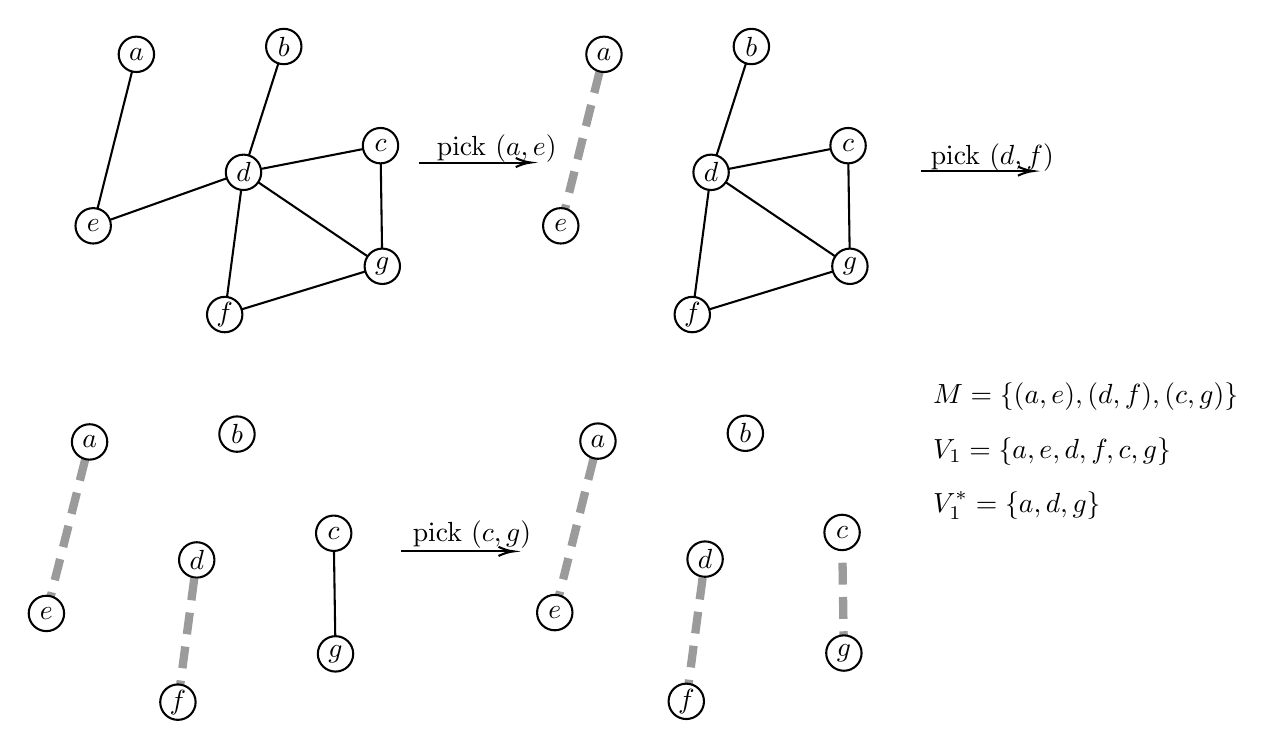
\begin{tikzpicture}[x=0.5pt,y=0.5pt,yscale=-1,xscale=1]
%uncomment if require: \path (0,509); %set diagram left start at 0, and has height of 509

%Straight Lines [id:da8273794433294758] 
\draw [color={rgb, 255:red, 155; green, 155; blue, 155 }  ,draw opacity=1 ][line width=3]  [dash pattern={on 7.88pt off 4.5pt}]  (386.16,427.29) -- (417.37,303.35) ;
%Straight Lines [id:da19729544641931185] 
\draw [color={rgb, 255:red, 155; green, 155; blue, 155 }  ,draw opacity=1 ][line width=3]  [dash pattern={on 7.88pt off 4.5pt}]  (481.2,491.42) -- (494.8,388.63) ;
%Straight Lines [id:da1947854045852928] 
\draw [color={rgb, 255:red, 155; green, 155; blue, 155 }  ,draw opacity=1 ][line width=3]  [dash pattern={on 7.88pt off 4.5pt}]  (595.1,456.53) -- (593.8,369.36) ;
%Straight Lines [id:da9648063665102072] 
\draw [color={rgb, 255:red, 155; green, 155; blue, 155 }  ,draw opacity=1 ][line width=3]  [dash pattern={on 7.88pt off 4.5pt}]  (113.81,492.01) -- (127.4,389.23) ;
%Straight Lines [id:da9576652196411746] 
\draw [color={rgb, 255:red, 155; green, 155; blue, 155 }  ,draw opacity=1 ][line width=3]  [dash pattern={on 7.88pt off 4.5pt}]  (18.77,427.89) -- (49.98,303.95) ;
%Straight Lines [id:da8239887263259694] 
\draw    (598.14,89.84) -- (499.14,109.11) ;
%Straight Lines [id:da8680955835635338] 
\draw    (485.54,211.9) -- (499.14,109.11) ;
%Straight Lines [id:da6116440428437093] 
\draw    (599.45,177.01) -- (485.54,211.9) ;
%Straight Lines [id:da2663821751343478] 
\draw    (599.45,177.01) -- (499.14,109.11) ;
%Straight Lines [id:da19351840074215054] 
\draw    (161.22,109.11) -- (260.22,89.84) ;
%Straight Lines [id:da43489413938826404] 
\draw    (161.22,109.11) -- (261.52,177.01) ;
%Straight Lines [id:da3853598268579197] 
\draw    (190.31,18.18) -- (161.22,109.11) ;
%Straight Lines [id:da21713072329995364] 
\draw    (261.52,177.01) -- (260.22,89.84) ;
%Straight Lines [id:da5478715757735835] 
\draw    (147.62,211.9) -- (261.52,177.01) ;
%Straight Lines [id:da42879006771456607] 
\draw    (52.58,147.77) -- (161.22,109.11) ;
%Straight Lines [id:da6771300098351073] 
\draw    (52.58,147.77) -- (83.79,23.83) ;
%Straight Lines [id:da4776548669152245] 
\draw    (147.62,211.9) -- (161.22,109.11) ;
%Shape: Ellipse [id:dp651117123053256] 
\draw  [fill={rgb, 255:red, 255; green, 255; blue, 255 }  ,fill opacity=1 ] (71,23.83) .. controls (71,16.77) and (76.73,11.04) .. (83.79,11.04) .. controls (90.86,11.04) and (96.58,16.77) .. (96.58,23.83) .. controls (96.58,30.9) and (90.86,36.62) .. (83.79,36.62) .. controls (76.73,36.62) and (71,30.9) .. (71,23.83) -- cycle ;
%Shape: Ellipse [id:dp7399561756845123] 
\draw  [fill={rgb, 255:red, 255; green, 255; blue, 255 }  ,fill opacity=1 ] (177.52,18.18) .. controls (177.52,11.11) and (183.25,5.39) .. (190.31,5.39) .. controls (197.38,5.39) and (203.1,11.11) .. (203.1,18.18) .. controls (203.1,25.24) and (197.38,30.97) .. (190.31,30.97) .. controls (183.25,30.97) and (177.52,25.24) .. (177.52,18.18) -- cycle ;
%Shape: Ellipse [id:dp8268258265249401] 
\draw  [fill={rgb, 255:red, 255; green, 255; blue, 255 }  ,fill opacity=1 ] (247.43,89.84) .. controls (247.43,82.78) and (253.15,77.05) .. (260.22,77.05) .. controls (267.28,77.05) and (273.01,82.78) .. (273.01,89.84) .. controls (273.01,96.9) and (267.28,102.63) .. (260.22,102.63) .. controls (253.15,102.63) and (247.43,96.9) .. (247.43,89.84) -- cycle ;
%Shape: Ellipse [id:dp5421818862330341] 
\draw  [fill={rgb, 255:red, 255; green, 255; blue, 255 }  ,fill opacity=1 ] (148.43,109.11) .. controls (148.43,102.05) and (154.15,96.32) .. (161.22,96.32) .. controls (168.28,96.32) and (174.01,102.05) .. (174.01,109.11) .. controls (174.01,116.18) and (168.28,121.9) .. (161.22,121.9) .. controls (154.15,121.9) and (148.43,116.18) .. (148.43,109.11) -- cycle ;
%Shape: Ellipse [id:dp45600813719389455] 
\draw  [fill={rgb, 255:red, 255; green, 255; blue, 255 }  ,fill opacity=1 ] (39.79,147.77) .. controls (39.79,140.71) and (45.52,134.98) .. (52.58,134.98) .. controls (59.64,134.98) and (65.37,140.71) .. (65.37,147.77) .. controls (65.37,154.84) and (59.64,160.56) .. (52.58,160.56) .. controls (45.52,160.56) and (39.79,154.84) .. (39.79,147.77) -- cycle ;
%Shape: Ellipse [id:dp031187496945339066] 
\draw  [fill={rgb, 255:red, 255; green, 255; blue, 255 }  ,fill opacity=1 ] (134.83,211.9) .. controls (134.83,204.83) and (140.56,199.11) .. (147.62,199.11) .. controls (154.69,199.11) and (160.41,204.83) .. (160.41,211.9) .. controls (160.41,218.96) and (154.69,224.69) .. (147.62,224.69) .. controls (140.56,224.69) and (134.83,218.96) .. (134.83,211.9) -- cycle ;
%Shape: Ellipse [id:dp7474313144054212] 
\draw  [fill={rgb, 255:red, 255; green, 255; blue, 255 }  ,fill opacity=1 ] (248.73,177.01) .. controls (248.73,169.94) and (254.46,164.22) .. (261.52,164.22) .. controls (268.59,164.22) and (274.31,169.94) .. (274.31,177.01) .. controls (274.31,184.07) and (268.59,189.8) .. (261.52,189.8) .. controls (254.46,189.8) and (248.73,184.07) .. (248.73,177.01) -- cycle ;
%Straight Lines [id:da10915523795701287] 
\draw    (528.24,18.18) -- (499.14,109.11) ;
%Straight Lines [id:da6013659372024278] 
\draw    (599.45,177.01) -- (598.14,89.84) ;
%Straight Lines [id:da2476997276246733] 
\draw [color={rgb, 255:red, 155; green, 155; blue, 155 }  ,draw opacity=1 ][line width=3]  [dash pattern={on 7.88pt off 4.5pt}]  (390.5,147.77) -- (421.72,23.83) ;
%Shape: Ellipse [id:dp27040633021074256] 
\draw  [fill={rgb, 255:red, 255; green, 255; blue, 255 }  ,fill opacity=1 ] (408.93,23.83) .. controls (408.93,16.77) and (414.65,11.04) .. (421.72,11.04) .. controls (428.78,11.04) and (434.51,16.77) .. (434.51,23.83) .. controls (434.51,30.9) and (428.78,36.62) .. (421.72,36.62) .. controls (414.65,36.62) and (408.93,30.9) .. (408.93,23.83) -- cycle ;
%Shape: Ellipse [id:dp9153562797015269] 
\draw  [fill={rgb, 255:red, 255; green, 255; blue, 255 }  ,fill opacity=1 ] (515.45,18.18) .. controls (515.45,11.11) and (521.17,5.39) .. (528.24,5.39) .. controls (535.3,5.39) and (541.03,11.11) .. (541.03,18.18) .. controls (541.03,25.24) and (535.3,30.97) .. (528.24,30.97) .. controls (521.17,30.97) and (515.45,25.24) .. (515.45,18.18) -- cycle ;
%Shape: Ellipse [id:dp47379487417600374] 
\draw  [fill={rgb, 255:red, 255; green, 255; blue, 255 }  ,fill opacity=1 ] (585.35,89.84) .. controls (585.35,82.78) and (591.07,77.05) .. (598.14,77.05) .. controls (605.2,77.05) and (610.93,82.78) .. (610.93,89.84) .. controls (610.93,96.9) and (605.2,102.63) .. (598.14,102.63) .. controls (591.07,102.63) and (585.35,96.9) .. (585.35,89.84) -- cycle ;
%Shape: Ellipse [id:dp7207828118279439] 
\draw  [fill={rgb, 255:red, 255; green, 255; blue, 255 }  ,fill opacity=1 ] (486.35,109.11) .. controls (486.35,102.05) and (492.08,96.32) .. (499.14,96.32) .. controls (506.2,96.32) and (511.93,102.05) .. (511.93,109.11) .. controls (511.93,116.18) and (506.2,121.9) .. (499.14,121.9) .. controls (492.08,121.9) and (486.35,116.18) .. (486.35,109.11) -- cycle ;
%Shape: Ellipse [id:dp7155442322771159] 
\draw  [fill={rgb, 255:red, 255; green, 255; blue, 255 }  ,fill opacity=1 ] (377.71,147.77) .. controls (377.71,140.71) and (383.44,134.98) .. (390.5,134.98) .. controls (397.57,134.98) and (403.29,140.71) .. (403.29,147.77) .. controls (403.29,154.84) and (397.57,160.56) .. (390.5,160.56) .. controls (383.44,160.56) and (377.71,154.84) .. (377.71,147.77) -- cycle ;
%Shape: Ellipse [id:dp4818001756043101] 
\draw  [fill={rgb, 255:red, 255; green, 255; blue, 255 }  ,fill opacity=1 ] (472.75,211.9) .. controls (472.75,204.83) and (478.48,199.11) .. (485.54,199.11) .. controls (492.61,199.11) and (498.33,204.83) .. (498.33,211.9) .. controls (498.33,218.96) and (492.61,224.69) .. (485.54,224.69) .. controls (478.48,224.69) and (472.75,218.96) .. (472.75,211.9) -- cycle ;
%Shape: Ellipse [id:dp9764479331484588] 
\draw  [fill={rgb, 255:red, 255; green, 255; blue, 255 }  ,fill opacity=1 ] (586.66,177.01) .. controls (586.66,169.94) and (592.38,164.22) .. (599.45,164.22) .. controls (606.51,164.22) and (612.24,169.94) .. (612.24,177.01) .. controls (612.24,184.07) and (606.51,189.8) .. (599.45,189.8) .. controls (592.38,189.8) and (586.66,184.07) .. (586.66,177.01) -- cycle ;
%Straight Lines [id:da7079754945425016] 
\draw    (227.71,457.12) -- (226.4,369.95) ;
%Shape: Ellipse [id:dp8120027238634924] 
\draw  [fill={rgb, 255:red, 255; green, 255; blue, 255 }  ,fill opacity=1 ] (37.19,303.95) .. controls (37.19,296.88) and (42.92,291.16) .. (49.98,291.16) .. controls (57.04,291.16) and (62.77,296.88) .. (62.77,303.95) .. controls (62.77,311.01) and (57.04,316.74) .. (49.98,316.74) .. controls (42.92,316.74) and (37.19,311.01) .. (37.19,303.95) -- cycle ;
%Shape: Ellipse [id:dp23465413123771173] 
\draw  [fill={rgb, 255:red, 255; green, 255; blue, 255 }  ,fill opacity=1 ] (143.71,298.29) .. controls (143.71,291.23) and (149.44,285.5) .. (156.5,285.5) .. controls (163.56,285.5) and (169.29,291.23) .. (169.29,298.29) .. controls (169.29,305.35) and (163.56,311.08) .. (156.5,311.08) .. controls (149.44,311.08) and (143.71,305.35) .. (143.71,298.29) -- cycle ;
%Shape: Ellipse [id:dp6697870946666823] 
\draw  [fill={rgb, 255:red, 255; green, 255; blue, 255 }  ,fill opacity=1 ] (213.61,369.95) .. controls (213.61,362.89) and (219.34,357.16) .. (226.4,357.16) .. controls (233.47,357.16) and (239.19,362.89) .. (239.19,369.95) .. controls (239.19,377.02) and (233.47,382.74) .. (226.4,382.74) .. controls (219.34,382.74) and (213.61,377.02) .. (213.61,369.95) -- cycle ;
%Shape: Ellipse [id:dp6678250120125151] 
\draw  [fill={rgb, 255:red, 255; green, 255; blue, 255 }  ,fill opacity=1 ] (114.61,389.23) .. controls (114.61,382.16) and (120.34,376.44) .. (127.4,376.44) .. controls (134.47,376.44) and (140.19,382.16) .. (140.19,389.23) .. controls (140.19,396.29) and (134.47,402.02) .. (127.4,402.02) .. controls (120.34,402.02) and (114.61,396.29) .. (114.61,389.23) -- cycle ;
%Shape: Ellipse [id:dp44880213332154095] 
\draw  [fill={rgb, 255:red, 255; green, 255; blue, 255 }  ,fill opacity=1 ] (5.98,427.89) .. controls (5.98,420.83) and (11.7,415.1) .. (18.77,415.1) .. controls (25.83,415.1) and (31.56,420.83) .. (31.56,427.89) .. controls (31.56,434.95) and (25.83,440.68) .. (18.77,440.68) .. controls (11.7,440.68) and (5.98,434.95) .. (5.98,427.89) -- cycle ;
%Shape: Ellipse [id:dp5261031453835676] 
\draw  [fill={rgb, 255:red, 255; green, 255; blue, 255 }  ,fill opacity=1 ] (101.02,492.01) .. controls (101.02,484.95) and (106.75,479.22) .. (113.81,479.22) .. controls (120.87,479.22) and (126.6,484.95) .. (126.6,492.01) .. controls (126.6,499.07) and (120.87,504.8) .. (113.81,504.8) .. controls (106.75,504.8) and (101.02,499.07) .. (101.02,492.01) -- cycle ;
%Shape: Ellipse [id:dp96264308088132] 
\draw  [fill={rgb, 255:red, 255; green, 255; blue, 255 }  ,fill opacity=1 ] (214.92,457.12) .. controls (214.92,450.06) and (220.65,444.33) .. (227.71,444.33) .. controls (234.77,444.33) and (240.5,450.06) .. (240.5,457.12) .. controls (240.5,464.18) and (234.77,469.91) .. (227.71,469.91) .. controls (220.65,469.91) and (214.92,464.18) .. (214.92,457.12) -- cycle ;
%Shape: Ellipse [id:dp08371522903251905] 
\draw  [fill={rgb, 255:red, 255; green, 255; blue, 255 }  ,fill opacity=1 ] (404.58,303.35) .. controls (404.58,296.29) and (410.31,290.56) .. (417.37,290.56) .. controls (424.44,290.56) and (430.16,296.29) .. (430.16,303.35) .. controls (430.16,310.42) and (424.44,316.14) .. (417.37,316.14) .. controls (410.31,316.14) and (404.58,310.42) .. (404.58,303.35) -- cycle ;
%Shape: Ellipse [id:dp16754302978302682] 
\draw  [fill={rgb, 255:red, 255; green, 255; blue, 255 }  ,fill opacity=1 ] (511.11,297.7) .. controls (511.11,290.63) and (516.83,284.91) .. (523.9,284.91) .. controls (530.96,284.91) and (536.69,290.63) .. (536.69,297.7) .. controls (536.69,304.76) and (530.96,310.48) .. (523.9,310.48) .. controls (516.83,310.48) and (511.11,304.76) .. (511.11,297.7) -- cycle ;
%Shape: Ellipse [id:dp8803652600651565] 
\draw  [fill={rgb, 255:red, 255; green, 255; blue, 255 }  ,fill opacity=1 ] (581.01,369.36) .. controls (581.01,362.3) and (586.73,356.57) .. (593.8,356.57) .. controls (600.86,356.57) and (606.59,362.3) .. (606.59,369.36) .. controls (606.59,376.42) and (600.86,382.15) .. (593.8,382.15) .. controls (586.73,382.15) and (581.01,376.42) .. (581.01,369.36) -- cycle ;
%Shape: Ellipse [id:dp08434869719365379] 
\draw  [fill={rgb, 255:red, 255; green, 255; blue, 255 }  ,fill opacity=1 ] (482.01,388.63) .. controls (482.01,381.57) and (487.74,375.84) .. (494.8,375.84) .. controls (501.86,375.84) and (507.59,381.57) .. (507.59,388.63) .. controls (507.59,395.7) and (501.86,401.42) .. (494.8,401.42) .. controls (487.74,401.42) and (482.01,395.7) .. (482.01,388.63) -- cycle ;
%Shape: Ellipse [id:dp8697258636657205] 
\draw  [fill={rgb, 255:red, 255; green, 255; blue, 255 }  ,fill opacity=1 ] (373.37,427.29) .. controls (373.37,420.23) and (379.1,414.5) .. (386.16,414.5) .. controls (393.23,414.5) and (398.95,420.23) .. (398.95,427.29) .. controls (398.95,434.36) and (393.23,440.08) .. (386.16,440.08) .. controls (379.1,440.08) and (373.37,434.36) .. (373.37,427.29) -- cycle ;
%Shape: Ellipse [id:dp3796179832525568] 
\draw  [fill={rgb, 255:red, 255; green, 255; blue, 255 }  ,fill opacity=1 ] (468.41,491.42) .. controls (468.41,484.35) and (474.14,478.63) .. (481.2,478.63) .. controls (488.27,478.63) and (493.99,484.35) .. (493.99,491.42) .. controls (493.99,498.48) and (488.27,504.21) .. (481.2,504.21) .. controls (474.14,504.21) and (468.41,498.48) .. (468.41,491.42) -- cycle ;
%Shape: Ellipse [id:dp22651898621493904] 
\draw  [fill={rgb, 255:red, 255; green, 255; blue, 255 }  ,fill opacity=1 ] (582.32,456.53) .. controls (582.32,449.46) and (588.04,443.74) .. (595.1,443.74) .. controls (602.17,443.74) and (607.89,449.46) .. (607.89,456.53) .. controls (607.89,463.59) and (602.17,469.32) .. (595.1,469.32) .. controls (588.04,469.32) and (582.32,463.59) .. (582.32,456.53) -- cycle ;
%Straight Lines [id:da8565598108716722] 
\draw    (287.8,102.04) -- (366.89,102.04) ;
\draw [shift={(368.89,102.04)}, rotate = 180] [color={rgb, 255:red, 0; green, 0; blue, 0 }  ][line width=0.75]    (10.93,-3.29) .. controls (6.95,-1.4) and (3.31,-0.3) .. (0,0) .. controls (3.31,0.3) and (6.95,1.4) .. (10.93,3.29)   ;
%Straight Lines [id:da8466299980928367] 
\draw    (650.72,108.21) -- (729.82,108.21) ;
\draw [shift={(731.82,108.21)}, rotate = 180] [color={rgb, 255:red, 0; green, 0; blue, 0 }  ][line width=0.75]    (10.93,-3.29) .. controls (6.95,-1.4) and (3.31,-0.3) .. (0,0) .. controls (3.31,0.3) and (6.95,1.4) .. (10.93,3.29)   ;
%Straight Lines [id:da6943383967058451] 
\draw    (275.35,383.05) -- (354.44,383.05) ;
\draw [shift={(356.44,383.05)}, rotate = 180] [color={rgb, 255:red, 0; green, 0; blue, 0 }  ][line width=0.75]    (10.93,-3.29) .. controls (6.95,-1.4) and (3.31,-0.3) .. (0,0) .. controls (3.31,0.3) and (6.95,1.4) .. (10.93,3.29)   ;

% Text Node
\draw (657.36,298.36) node [anchor=north west][inner sep=0.75pt]   [align=left] {$\displaystyle V_{1} =\{a,e,d,f,c,g\}$};
% Text Node
\draw (657.36,337.59) node [anchor=north west][inner sep=0.75pt]   [align=left] {$\displaystyle V^{*}_{1} =\{a,d,g\}$};
% Text Node
\draw (83.79,23.83) node   [align=left] {$\displaystyle a$};
% Text Node
\draw (190.31,18.18) node   [align=left] {$\displaystyle b$};
% Text Node
\draw (260.22,89.84) node   [align=left] {$\displaystyle c$};
% Text Node
\draw (161.22,109.11) node   [align=left] {$\displaystyle d$};
% Text Node
\draw (52.58,147.77) node   [align=left] {$\displaystyle e$};
% Text Node
\draw (147.62,211.9) node   [align=left] {$\displaystyle f$};
% Text Node
\draw (261.52,177.01) node   [align=left] {$\displaystyle g$};
% Text Node
\draw (421.72,23.83) node   [align=left] {$\displaystyle a$};
% Text Node
\draw (528.24,18.18) node   [align=left] {$\displaystyle b$};
% Text Node
\draw (598.14,89.84) node   [align=left] {$\displaystyle c$};
% Text Node
\draw (499.14,109.11) node   [align=left] {$\displaystyle d$};
% Text Node
\draw (390.5,147.77) node   [align=left] {$\displaystyle e$};
% Text Node
\draw (485.54,211.9) node   [align=left] {$\displaystyle f$};
% Text Node
\draw (599.45,177.01) node   [align=left] {$\displaystyle g$};
% Text Node
\draw (49.98,303.95) node   [align=left] {$\displaystyle a$};
% Text Node
\draw (156.5,298.29) node   [align=left] {$\displaystyle b$};
% Text Node
\draw (226.4,369.95) node   [align=left] {$\displaystyle c$};
% Text Node
\draw (127.4,389.23) node   [align=left] {$\displaystyle d$};
% Text Node
\draw (18.77,427.89) node   [align=left] {$\displaystyle e$};
% Text Node
\draw (113.81,492.01) node   [align=left] {$\displaystyle f$};
% Text Node
\draw (227.71,457.12) node   [align=left] {$\displaystyle g$};
% Text Node
\draw (417.37,303.35) node   [align=left] {$\displaystyle a$};
% Text Node
\draw (523.9,297.7) node   [align=left] {$\displaystyle b$};
% Text Node
\draw (593.8,369.36) node   [align=left] {$\displaystyle c$};
% Text Node
\draw (494.8,388.63) node   [align=left] {$\displaystyle d$};
% Text Node
\draw (386.16,427.29) node   [align=left] {$\displaystyle e$};
% Text Node
\draw (481.2,491.42) node   [align=left] {$\displaystyle f$};
% Text Node
\draw (595.1,456.53) node   [align=left] {$\displaystyle g$};
% Text Node
\draw (298.71,79.84) node [anchor=north west][inner sep=0.75pt]   [align=left] {pick $\displaystyle ( a,e)$};
% Text Node
\draw (655.68,86.01) node [anchor=north west][inner sep=0.75pt]   [align=left] {pick $\displaystyle ( d,f)$};
% Text Node
\draw (281.28,358.84) node [anchor=north west][inner sep=0.75pt]   [align=left] {pick $\displaystyle ( c,g)$};
% Text Node
\draw (657.36,259.13) node [anchor=north west][inner sep=0.75pt]   [align=left] {$\displaystyle M=\{( a,e) ,( d,f) ,( c,g)\}$};


\end{tikzpicture}

